Este trabalho adota a \emph{Design Science Research} (DSR) como metodologia de pesquisa, uma abordagem focada na concepção, desenvolvimento e avaliação de artefatos tecnológicos para solucionar problemas práticos e relevantes \cite{hevner2004designscienceinformation, dresch2015distinctiveanalysiscase}. O artefato central desenvolvido neste projeto é uma plataforma robótica móvel de baixo custo, baseada em Raspberry Pi, ROS 2 e câmera RGB-D, voltada à execução e avaliação de SLAM visual embarcado em ambiente interno.

Para uma formalização acadêmica, a pesquisa também é classificada conforme a taxonomia de Prodanov e Freitas \cite{prodanov2012metodologiatrabalhocientifico}, detalhada na Seção \ref{sec:Class_Pesquisa}. As etapas práticas do desenvolvimento, alinhadas à DSR, são descritas na Seção \ref{sec:etapas_dsr}.

\section{Classificação da Pesquisa}\label{sec:Class_Pesquisa}

Com base na obra de Prodanov e Freitas \cite{prodanov2012metodologiatrabalhocientifico}, a presente pesquisa é classificada quanto à sua natureza, seus objetivos, seus procedimentos técnicos e à forma de abordagem do problema.

\noindent\textbf{Quanto à Natureza}\par
Do ponto de vista de sua natureza, esta pesquisa classifica-se como \textbf{Pesquisa Aplicada}. Segundo os autores, a pesquisa aplicada ``objetiva gerar conhecimentos para aplicação prática dirigidos à solução de problemas específicos'' \cite[p. 51]{prodanov2012metodologiatrabalhocientifico}. O trabalho se enquadra nesta definição porque busca desenvolver e avaliar uma solução tecnológica concreta para um problema prático: a integração de sensores, controle embarcado e SLAM visual em uma plataforma robótica física de baixo custo.

\noindent\textbf{Quanto aos Objetivos}\par
No que se refere aos seus objetivos, a pesquisa combina características \textbf{exploratórias}, \textbf{descritivas} e \textbf{explicativas}.
\begin{itemize}
    \item \textbf{Pesquisa Exploratória:} A pesquisa possui caráter exploratório na investigação das limitações práticas de executar SLAM visual em hardware restrito, bem como na identificação dos ajustes necessários de sensores, referenciais e parâmetros do RTAB-Map.
    \item \textbf{Pesquisa Descritiva:} A pesquisa assume viés descritivo ao registrar a arquitetura construída, os fluxos de tópicos ROS 2, as evidências de integração e as métricas observadas durante os testes controlados.
    \item \textbf{Pesquisa Explicativa:} A análise busca explicar como fatores como odometria, ruído da IMU, taxa de processamento, perda de pose e configuração das transformações influenciam a estabilidade do mapeamento visual.
\end{itemize}

\noindent\textbf{Quanto aos Procedimentos Técnicos}\par
Considerando os procedimentos técnicos, esta pesquisa classifica-se como \textbf{Pesquisa Bibliográfica} e \textbf{Pesquisa Experimental}.
\begin{itemize}
    \item \textbf{Pesquisa Bibliográfica:} É desenvolvida ``a partir de material já publicado'' \cite[p. 54]{prodanov2012metodologiatrabalhocientifico}, sendo utilizada para fundamentar as decisões sobre SLAM visual, sensores RGB-D, computação embarcada, ROS 2 e fusão sensorial.
    \item \textbf{Pesquisa Experimental:} É o procedimento central do trabalho, pois envolve a definição de variáveis de observação, execução de testes controlados e análise do comportamento do artefato físico. O objeto de estudo é o desempenho do pipeline de SLAM embarcado no robô real, não a comparação com ambiente simulado ou processamento remoto.
\end{itemize}

\noindent\textbf{Quanto à Forma de Abordagem do Problema}\par
A abordagem do problema é predominantemente \textbf{Quantitativa}, com elementos de análise \textbf{Qualitativa}.
\begin{itemize}
    \item \textbf{Pesquisa Quantitativa:} A avaliação considera dados mensuráveis, como frequência dos tópicos, taxa de processamento, uso de CPU e memória, ocorrência de perda de pose, estabilidade do mapa e comportamento da odometria antes e depois de ajustes no pipeline.
    \item \textbf{Pesquisa Qualitativa:} A análise qualitativa é empregada para interpretar a coerência visual do mapa, a consistência das transformações entre referenciais, os sintomas de falhas de rastreamento e as limitações práticas observadas durante os ensaios.
\end{itemize}

\section{Etapas da Pesquisa (DSR)}
\label{sec:etapas_dsr}

Enquanto a Seção \ref{sec:Class_Pesquisa} classificou a pesquisa de forma taxonômica, esta seção detalha o processo metodológico prático. Este trabalho é conduzido pela \emph{Design Science Research} (DSR) \cite{hevner2004designscienceinformation, dresch2015distinctiveanalysiscase}, uma metodologia focada na concepção, construção e avaliação de um artefato tecnológico para solucionar um problema prático.

O problema prático, conforme definido na Introdução, é a dificuldade de integrar sensores e executar SLAM visual em uma plataforma robótica física de baixo custo, sujeita a limitações de processamento, ruído sensorial, restrições de alimentação e inconsistências de odometria. O artefato desenvolvido é, portanto, uma arquitetura física e lógica de robô móvel capaz de adquirir dados RGB-D e inerciais, publicar os tópicos necessários no ROS 2, estimar movimento e gerar mapas por meio do RTAB-Map.

O processo de DSR é organizado em três etapas iterativas. A Figura \ref{fig:fluxo_metodologia} ilustra o fluxo metodológico adotado, detalhando as atividades específicas de cada fase e o ciclo de realimentação entre validação experimental e ajustes do artefato.

\begin{figure}[H]
    \centering
    \caption{Fluxograma das etapas da metodologia DSR aplicadas ao projeto}
    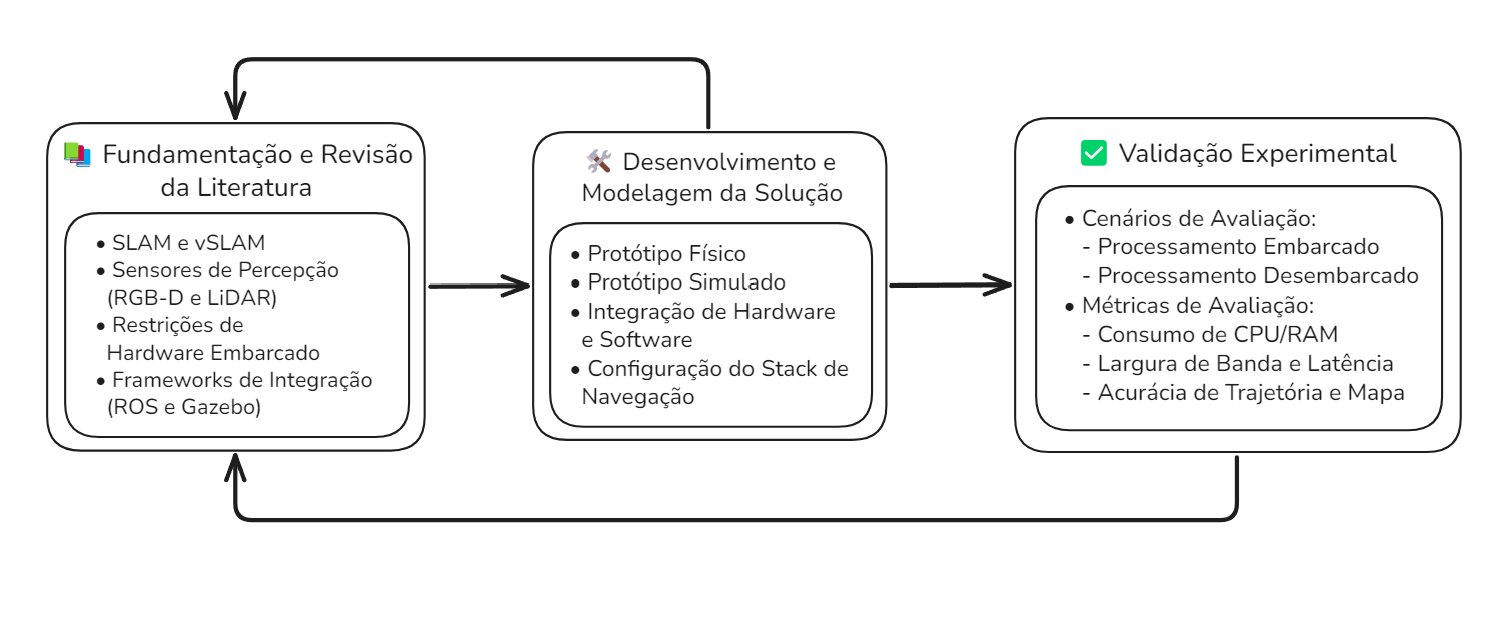
\includegraphics[width=1.0\textwidth]{figuras/fluxoDSR.png}
    \label{fig:fluxo_metodologia}
    Elaborado pelo autor (2025).
\end{figure}

As etapas ilustradas são descritas detalhadamente nas subseções a seguir.

\subsection{Etapa 1: Fundamentação e Revisão da Literatura}
\label{ssec:etapa1_revisao}

A primeira etapa consiste na investigação teórica para identificar a lacuna de pesquisa e fundamentar as decisões de projeto do artefato. Esta revisão abrange quatro pilares centrais:

\begin{enumerate}
     \item \textbf{SLAM e vSLAM:} Estudo dos fundamentos teóricos do SLAM e de sua variação visual, com foco na utilização de imagens RGB-D para estimativa de pose, fechamento de ciclo e geração de mapas \cite{taheri2021slamdefinitionevolution, guapacha2017localizacaomapeamentosimultaneos}.

    \item \textbf{Sensores de Percepção e Odometria:} Análise da câmera RGB-D como sensor principal de percepção e da IMU/odometria das rodas como fontes auxiliares de movimento. Esta etapa inclui o estudo de limitações de campo de visão, ruído, desfoque de movimento e possibilidades de fusão sensorial \cite{kamarudin2015improvingperformance2d, qayyum2017imuaidedrgbd}.

    \item \textbf{Hardware Embarcado:} Investigação dos desafios de implementar vSLAM em \textit{Single Board Computers} de baixo custo, como o Raspberry Pi \cite{raspberrypi2019raspberrypi}, considerando gargalos de CPU, memória, largura de banda e aquecimento \cite{costa2019characterizingpolybenchgpu, canovas2021onboarddynamicrgbd}.
    
    \item \textbf{Frameworks de Integração:} Estudo do ROS 2 como \emph{middleware} para integração de nós, sensores, atuadores, tópicos e transformações. O RTAB-Map é analisado como biblioteca principal de SLAM visual, e ferramentas de visualização como RViz são utilizadas para inspeção dos dados publicados.
\end{enumerate}

\subsection{Etapa 2: Desenvolvimento e Integração do Artefato}
\label{ssec:etapa2_artefato}

Esta etapa constitui o núcleo prático da pesquisa e é detalhada no Capítulo \ref{cap-desenvolvimento}. O desenvolvimento concentra-se na construção e integração do protótipo físico, adotando uma abordagem incremental para reduzir riscos técnicos antes da avaliação final.

As fases de desenvolvimento são:

\begin{itemize}
    \item \textbf{Montagem e Integração de Hardware:} Reaproveitamento do chassi de robô móvel, instalação do Raspberry Pi, microcontrolador, ponte H, bateria, câmera RGB-D e IMU.

    \item \textbf{Desenvolvimento do Firmware de Baixo Nível:} Implementação da interface responsável por receber comandos de velocidade, acionar os motores e transmitir leituras da IMU para a unidade de processamento.
    
    \item \textbf{Configuração do Ambiente Embarcado:} Instalação e configuração do Ubuntu Server, ROS 2, drivers da câmera RGB-D, comunicação serial, teleoperação e \textit{middleware} de comunicação.

    \item \textbf{Integração do Pipeline de SLAM:} Organização dos tópicos de imagem, profundidade, IMU, odometria e transformações necessárias para execução do RTAB-Map no Raspberry Pi.
    
    \item \textbf{Ajustes de Odometria e Fusão Sensorial:} Avaliação de inconsistências entre odometria das rodas, IMU e pose estimada pelo SLAM, incluindo a possibilidade de uso de filtro de Kalman estendido para fusão de dados.
\end{itemize}

Simulação e processamento remoto não compõem o eixo de avaliação desta versão do trabalho. Quando mencionados, são tratados apenas como referências de contexto ou possibilidades externas ao escopo atual.

\subsection{Etapa 3: Protocolo de Validação Experimental}
\label{ssec:etapa3_validacao}

A etapa final consiste na definição e execução de experimentos controlados no protótipo físico para avaliar o comportamento do artefato e responder à questão de pesquisa. A validação concentra-se na estabilidade do pipeline de SLAM visual embarcado e na capacidade do sistema de produzir dados coerentes para mapeamento em ambiente interno, enfrentando as limitações físicas do hardware selecionado.

O protocolo experimental contempla os seguintes cenários:

\begin{enumerate}
    \item \textbf{Teste de Integração dos Sensores:} Verificação da publicação dos tópicos de câmera RGB-D, IMU, odometria e comandos de velocidade, incluindo frequência média e estabilidade temporal.

    \item \textbf{Teste de Teleoperação Controlada:} Deslocamento manual do robô em trajetórias simples, como movimentos retilíneos, rotações e percursos curtos em ambiente interno, para observar resposta dos motores e consistência da odometria.
    
    \item \textbf{Execução do RTAB-Map Embarcado:} Avaliação do comportamento do SLAM visual no Raspberry Pi, registrando perda de pose, taxa de atualização, estabilidade do mapa e coerência entre trajetória estimada e movimento observado.

    \item \textbf{Avaliação de Ajustes de Odometria/Fusão Sensorial:} Comparação do comportamento do pipeline antes e depois de ajustes de parâmetros ou fusão entre IMU e odometria das rodas, quando esta etapa estiver concluída.
\end{enumerate}

Para avaliar a arquitetura proposta, serão coletadas métricas computacionais e métricas de qualidade da localização/mapeamento. Além das métricas quantitativas, será realizada avaliação qualitativa do mapa gerado. Os dados serão incorporados ao texto apenas após validação dos artefatos experimentais, evitando que esta versão parcial apresente conclusões antes da consolidação dos testes.

\begin{itemize}
    \item \textbf{Métricas de Desempenho Computacional:} Uso de CPU, uso de memória RAM, taxa de publicação dos tópicos de imagem/profundidade, taxa de processamento do SLAM e ocorrência de instabilidade térmica.
    \item \textbf{Métricas de Consistência do Pipeline:} Frequência de IMU e odometria, continuidade das transformações TF, ausência de falhas de sincronização e estabilidade da pose estimada.
    \item \textbf{Métricas de Qualidade do SLAM:} Ocorrência de perda de rastreamento, coerência visual do mapa, completude de áreas mapeadas, presença de deformações e estabilidade após fechamento de ciclo quando aplicável.
\end{itemize}

Os resultados quantitativos e evidências visuais serão consolidados no Capítulo \ref{cap-resultados-discussao}. Quando uma métrica ainda depender de coleta experimental, ela será tratada como evidência a consolidar, evitando conclusões antecipadas.
